\documentclass[10pt,dvipsnames]{beamer}
\usepackage[T1]{fontenc}
\usepackage{libertinus}
\usepackage{amsmath}
\usepackage[most]{tcolorbox}
\usepackage{graphicx}

\usepackage{hyperref}
%python 
\usepackage{listings}
% Default fixed font does not support bold face
\DeclareFixedFont{\ttb}{T1}{txtt}{bx}{n}{8} % for bold
\DeclareFixedFont{\ttm}{T1}{txtt}{m}{n}{8}  % for normal

% Custom colors
\usepackage{color}
\definecolor{deepblue}{rgb}{0,0,0.5}
\definecolor{deepred}{rgb}{0.6,0,0}
\definecolor{deepgreen}{rgb}{0,0.5,0}

\usepackage{listings}

% Python style for highlighting
\newcommand\pythonstyle{\lstset{
		language=Python,
		basicstyle=\ttm,
		morekeywords={self},              % Add keywords here
		keywordstyle=\ttb\color{deepblue},
		emph={MyClass,__init__},          % Custom highlighting
		emphstyle=\ttb\color{deepred},    % Custom highlighting style
		stringstyle=\color{deepgreen},
		frame=tb,                         % Any extra options here
		showstringspaces=false
}}


% Python environment
\lstnewenvironment{python}[1][]
{
	\pythonstyle
	\lstset{#1}
}
{}

% Python for external files
\newcommand\pythonexternal[2][]{{
		\pythonstyle
		\lstinputlisting[#1]{#2}}}

% Python for inline
\newcommand\pythoninline[1]{{\pythonstyle\lstinline!#1!}}

\usepackage{xcolor}  
\newcommand{\cb}[1]{{\color{CadetBlue}#1}}

\usepackage{pgfplots}
\pgfplotsset{compat=newest}
\setlength{\parskip}{0.5em}

\usepackage{setspace}
\setstretch{1.25}  
\usetheme{Singapore}
\setbeamertemplate{navigation symbols}{}

\setbeamertemplate{footline}{
    \leavevmode%
    \hbox{%
        \begin{beamercolorbox}[wd=.5\paperwidth,ht=2.25ex,dp=1ex,center]{author in head/foot}%
            % Customize this part if you want to add author or date information
        \end{beamercolorbox}%
        \begin{beamercolorbox}[wd=.5\paperwidth,ht=2.25ex,dp=1ex,right]{title in head/foot}%
            \usebeamerfont{title in head/foot}\insertframenumber{} / \inserttotalframenumber\hspace*{2ex} 
        \end{beamercolorbox}}%
    \vskip0pt%
}

\title{CSE574 Introduction to Machine Learning}
\subtitle{Clustering}
\author{Jue Guo}
\institute{University at Buffalo}
\date{\today}

\begin{document}
\begin{frame}
    \titlepage
\end{frame}
\begin{frame}
    \frametitle{Outline}
    \tableofcontents
\end{frame}

\section{k-means clustering}
\begin{frame}
    \frametitle{Learning Objective}
    \begin{itemize}
        \item Define clustering.
        \item Calculate cluster centroids and inertia.
        \item List steps in the k-means clustering algorithm.
        \item Use the elbow and silhouette methods to select the optimal number of clusters.
    \end{itemize}
\end{frame}

\subsection{Clustering}
\begin{frame}
    \frametitle{Clustering}
    \textbf{Clustering} is an unsupervised learning task in which instances are grouped based on similarities in the input features.
    \begin{itemize}
        \item Since clustering is unsupervised, no target output features exist. Instead, clustering results in a new feature containing group assignments.
    \end{itemize}
    Clustering algorithms use similarity measures to group instances, such as distance or correlation. Applications of clustering include customer segmentation, recommendation systems, and social network analysis.
\end{frame}

\begin{frame}
    \frametitle{Clustering grocery customers.}
    \begin{figure}[ht]
        \centering
        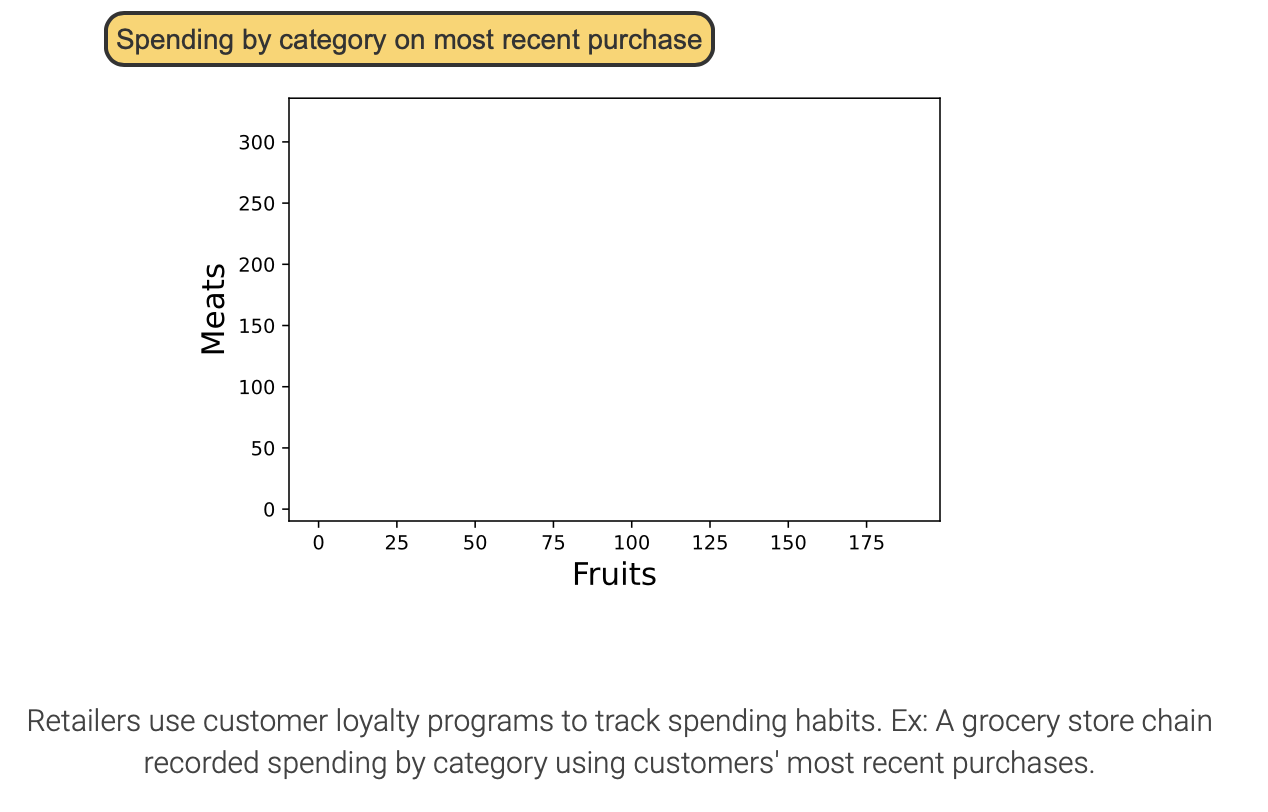
\includegraphics[width=0.8\textwidth]{imgs/k_mean_1.png}
    \end{figure}
\end{frame}

\begin{frame}
    \frametitle{Clustering grocery customers.}
    \begin{figure}[ht]
        \centering
        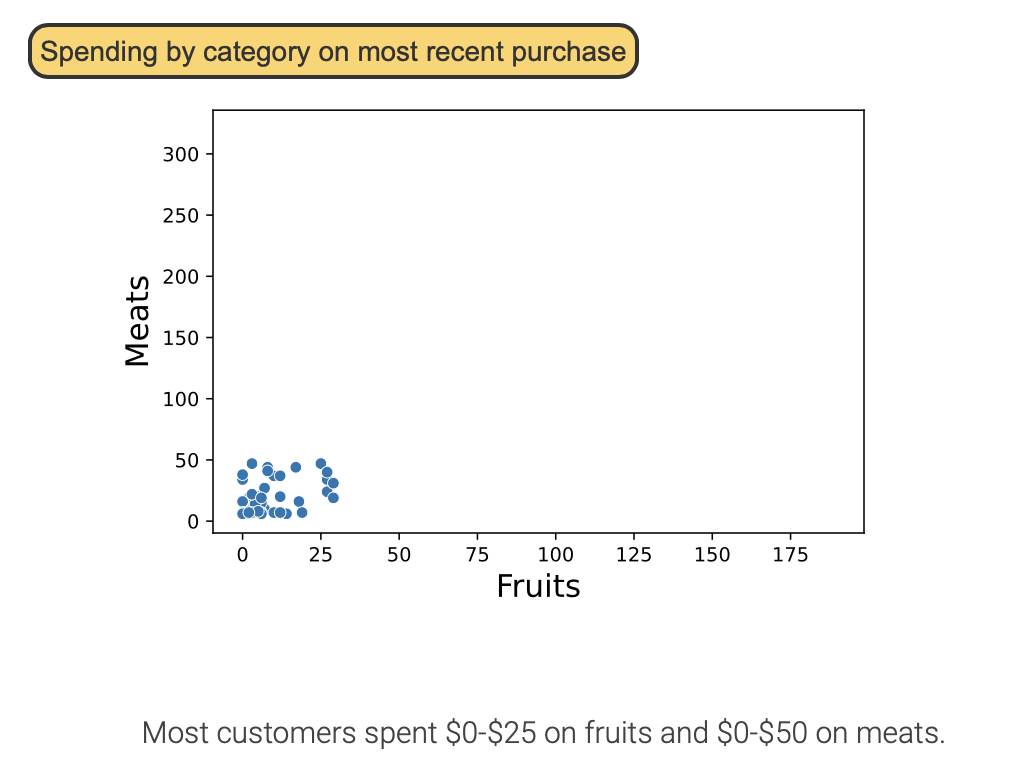
\includegraphics[width=0.8\textwidth]{imgs/k_mean_2.png}
    \end{figure}
\end{frame}

\begin{frame}
    \frametitle{Clustering grocery customers.}
    \begin{figure}[ht]
        \centering
        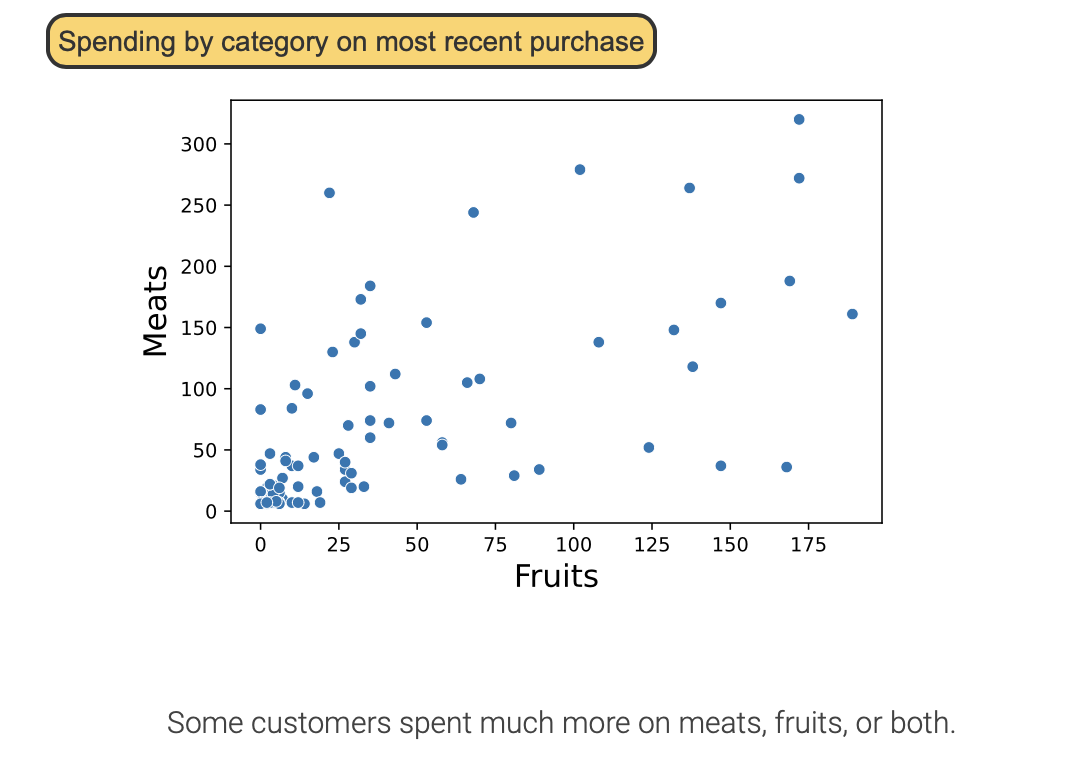
\includegraphics[width=0.8\textwidth]{imgs/k_mean_3.png}
    \end{figure}
\end{frame}

\begin{frame}
    \frametitle{Clustering grocery customers.}
    \begin{figure}[ht]
        \centering
        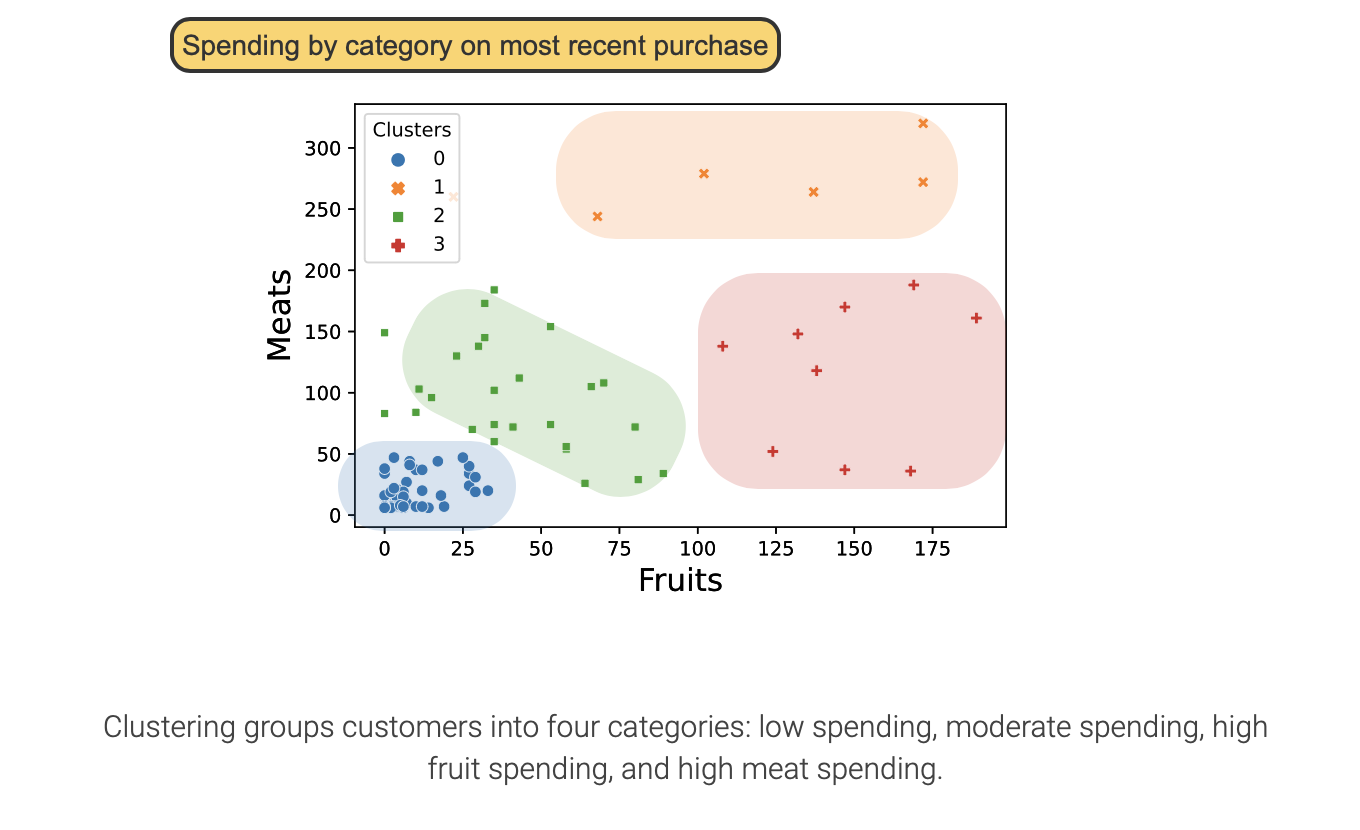
\includegraphics[width=0.8\textwidth]{imgs/k_mean_4.png}
    \end{figure}
\end{frame}

\begin{frame}
    \frametitle{Clustering grocery customers.}
    \begin{figure}[ht]
        \centering
        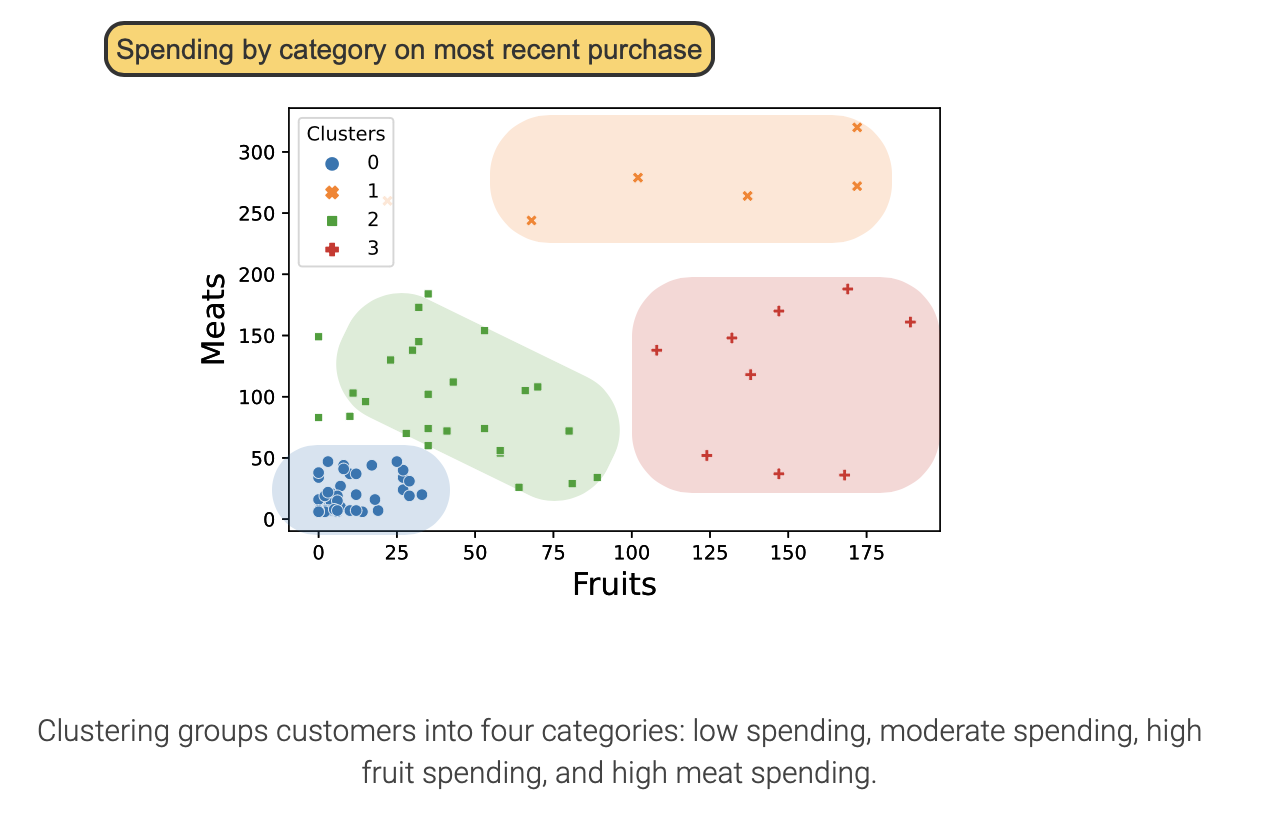
\includegraphics[width=0.8\textwidth]{imgs/k_mean_5.png}
    \end{figure}
\end{frame}
\subsection{Cluster centroids}
\begin{frame}
    \frametitle{Cluster centroids}

    The \textbf{centroid} of a cluster is the mean position of the cluster's instances. Centroids are used to summarize the position of the cluster and
    assign instances to clusters. For a cluster $C_{i}$, the centroid's value is:
    $$
        \overline{\mathbf{x}_{i}}=\frac{\sum_{j \in C_{i}} \mathbf{x}_{j}}{n_{i}}
    $$
    where $\mathbf{x}_{j}$ is a $p$-dimensional input vector containing the input feature values for instance $j$ and $n_{i}$ is the number of instances in cluster $k$.

\end{frame}

\begin{frame}
    \frametitle{Cluster centroids}
    The \textbf{inertia} of a cluster is the average of each instance's squared distance to the centroid. For cluster $i$, the inertia is:
    $$
        I_{i}=\frac{\sum_{j \in C_{i}}\left|\mathbf{x}_{j}-\overline{\mathbf{x}_{i}}\right|^{2}}{n_{i}}
    $$
    Inertia is also called the cluster's sum of squares. Clusters with low inertia contain more similar instances than clusters with high inertia.
\end{frame}

\begin{frame}
    \frametitle{Calculating centroids and inertia.}
    \begin{figure}[ht]
        \centering
        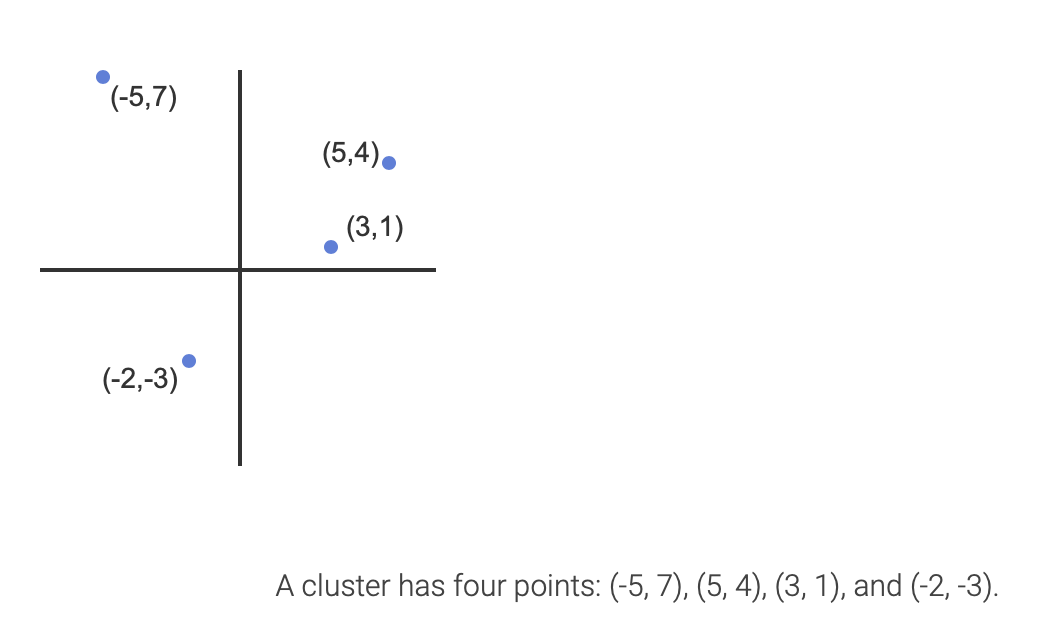
\includegraphics[width=0.8\textwidth]{imgs/k_mean_6.png}
    \end{figure}
\end{frame}

\begin{frame}
    \frametitle{Calculating centroids and inertia.}
    \begin{figure}[ht]
        \centering
        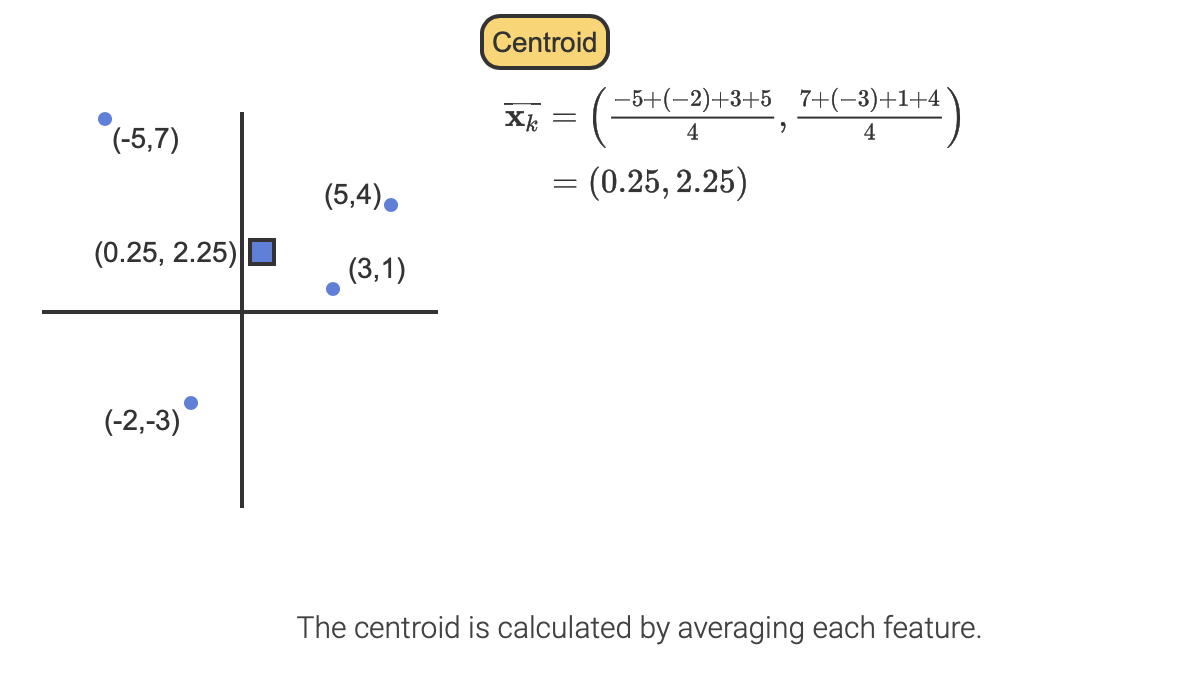
\includegraphics[width=0.8\textwidth]{imgs/k_mean_7.png}
    \end{figure}
\end{frame}

\begin{frame}
    \frametitle{Calculating centroids and inertia.}
    \begin{figure}[ht]
        \centering
        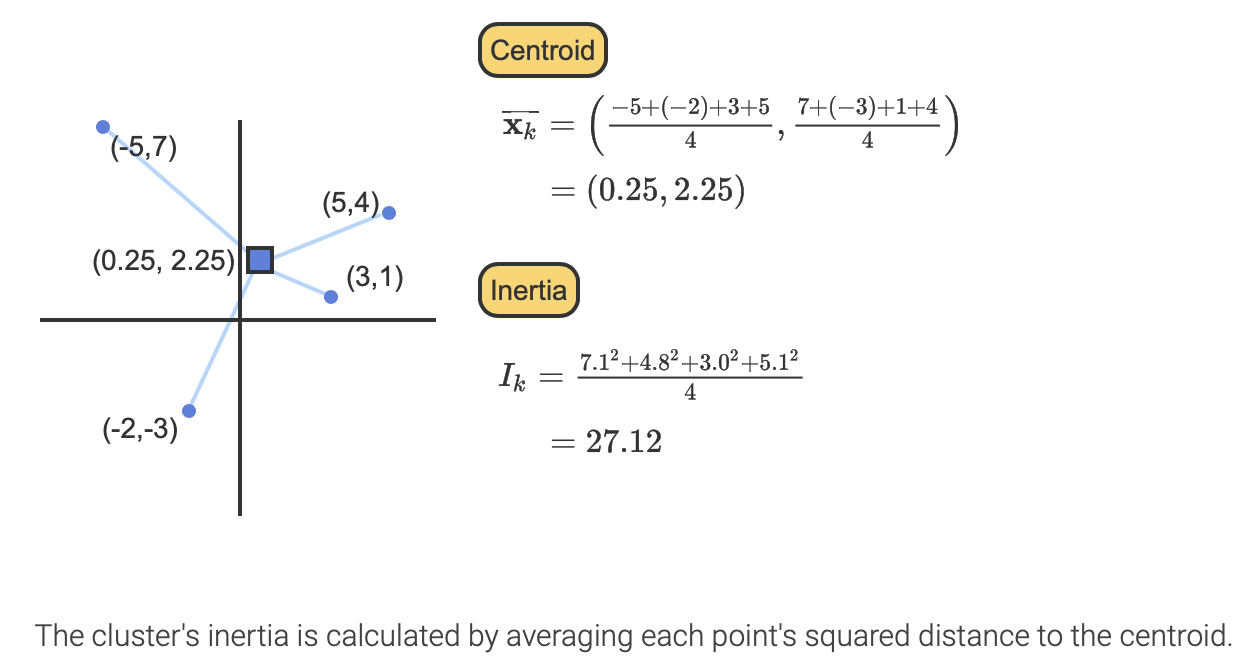
\includegraphics[width=0.8\textwidth]{imgs/k_mean_8.png}
    \end{figure}
\end{frame}

\subsection{k-means clustering}
\begin{frame}
    \frametitle{k-means clustering}
    \textbf{k-means clustering} is a clustering algorithm that assigns instances into the cluster with the nearest centroid.
    \begin{itemize}
        \item In k-means clustering, the number of clusters, \(k\), is chosen in advance. k-means clustering is considered stable if the final cluster assignment does not depend on the starting clusters.
        \item But, stability is not guaranteed, especially when no clear separation between instances exists.
    \end{itemize}
\end{frame}

\begin{frame}
    \frametitle{k-means clustering}

    Randomly select $k$ points for the initial centroids.
    \begin{enumerate}
        \item Assign each instance to the nearest center.
        \item Calculate the new cluster centroid.
        \item Continue until the cluster centroids do not change or the maximum number of iterations is reached.
    \end{enumerate}
\end{frame}

\subsection{Select the optimal number of clusters}
\begin{frame}
    \frametitle{Selecting the optimal number of clusters}
    Two common methods for choosing the optimal value of $k$ for a dataset are the elbow method and silhouette method.
    \begin{itemize}
        \item The \textbf{elbow method} graphs the total inertia of the clusters against values of $k$ and chooses the $k$ for which the curve levels off. Since increasing $k$ also increases model complexity, the elbow method finds the $k$ with the best tradeoff between complexity and inertia.
    \end{itemize}
\end{frame}

\begin{frame}
    \frametitle{Selecting the optimal number of clusters}
    The \textbf{silhouette method} calculates the silhouette coefficient for each instance, and chooses the $k$ with the highest mean silhouette score.
    \begin{itemize}
        \item For instance $j$, the silhouette coefficient is
              $$
                  S(j)=\frac{\overline{d_{o u t}(j)}-\overline{d_{i n}(j)}}{\max \left(\overline{d_{o u t}(j)}, \overline{d_{i n}(j)}\right)}
              $$
              where $\overline{d_{\text {out }}(j)}$ is the average distance of instance $i$ to the centroid of all other clusters, and $\overline{d_{i n}(j)}$ is the average distance of instance $i$ to all other instances in instance $i$ 's cluster. Silhouette coefficients range from -1 to +1 : An instance with a high silhouette coefficient is close to its own centroid, but far from the other centroids.
    \end{itemize}
\end{frame}

\begin{frame}
    \frametitle{Silhouette Plots}
    \textbf{Silhouette plots} graph the silhouette coefficient for each instance, grouped by cluster. Values of $k$ for which some clusters have all below-average silhouette coefficients, or a high proportion of negative silhouette coefficients, should not be used.
\end{frame}

\begin{frame}
    \frametitle{}
    \begin{figure}[ht]
        \centering
        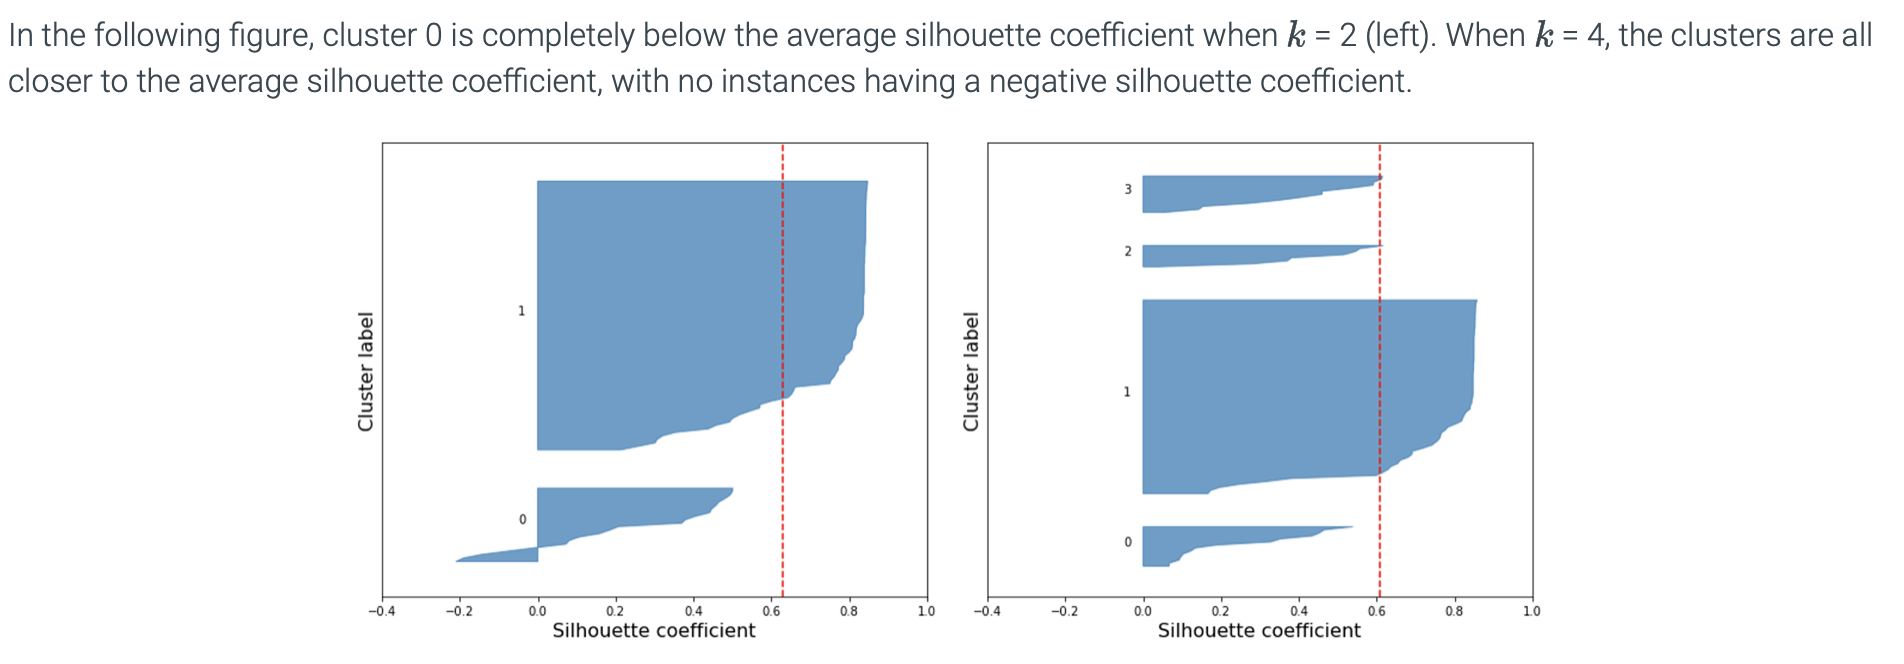
\includegraphics[width=0.8\textwidth]{imgs/k_mean_9.png}
        \caption{Silhouette plots for customer spending data.}
    \end{figure}
\end{frame}

\begin{frame}
    \frametitle{Selecting the optimal number of clusters.}
    \begin{figure}[ht]
        \centering
        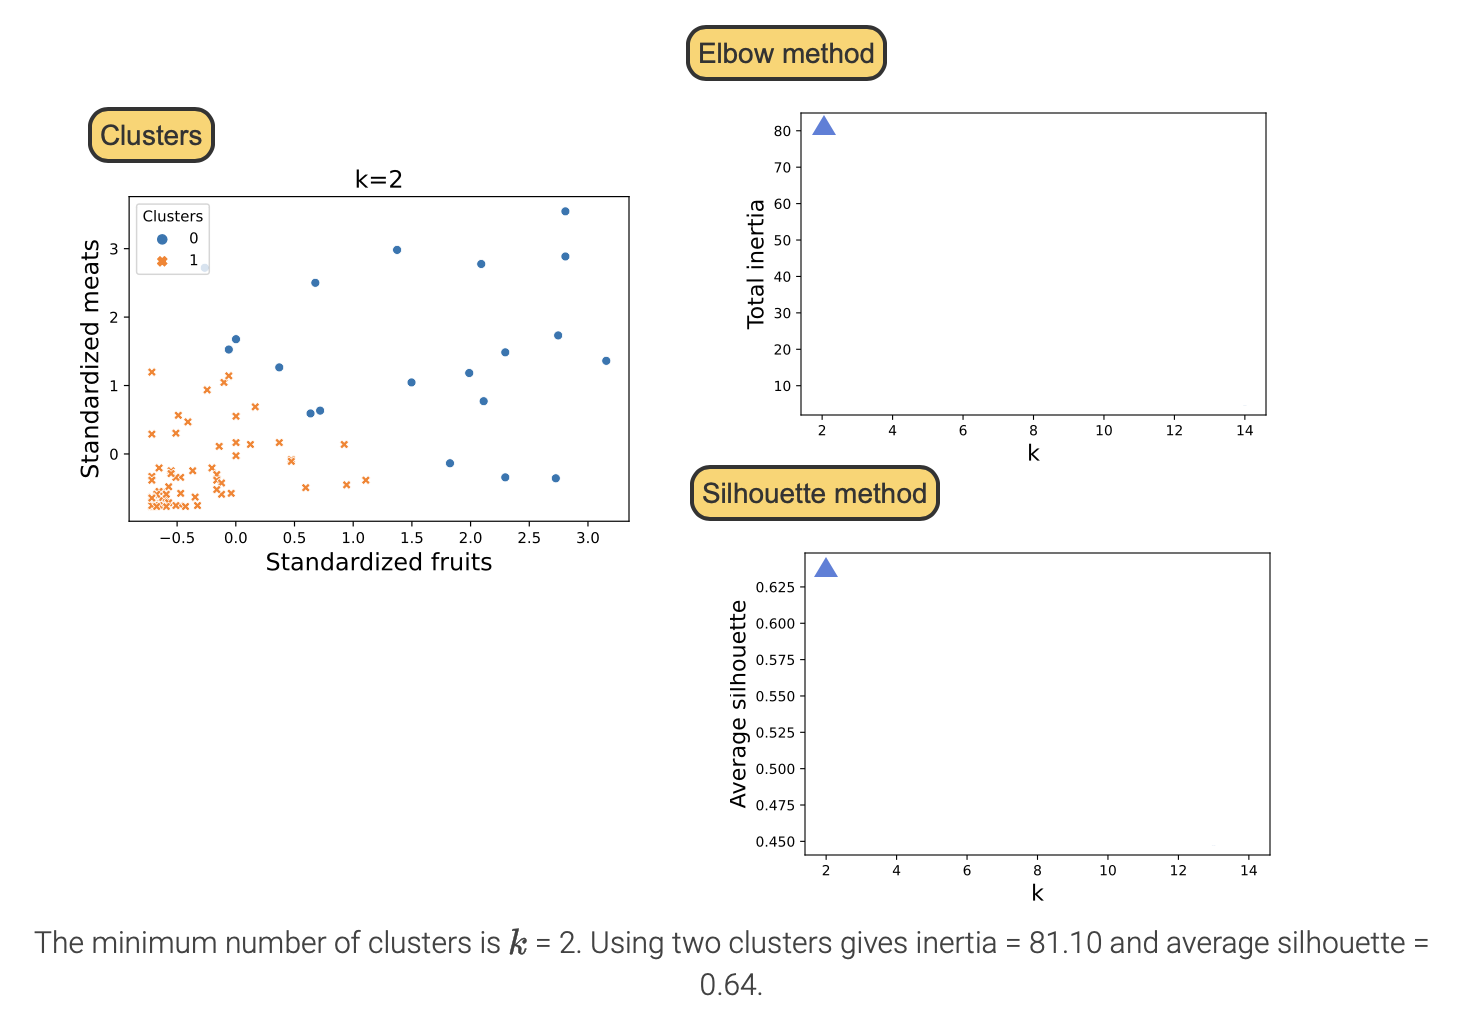
\includegraphics[width=0.8\textwidth]{imgs/k_mean_10.png}
    \end{figure}
\end{frame}

\begin{frame}
    \frametitle{Selecting the optimal number of clusters.}
    \begin{figure}[ht]
        \centering
        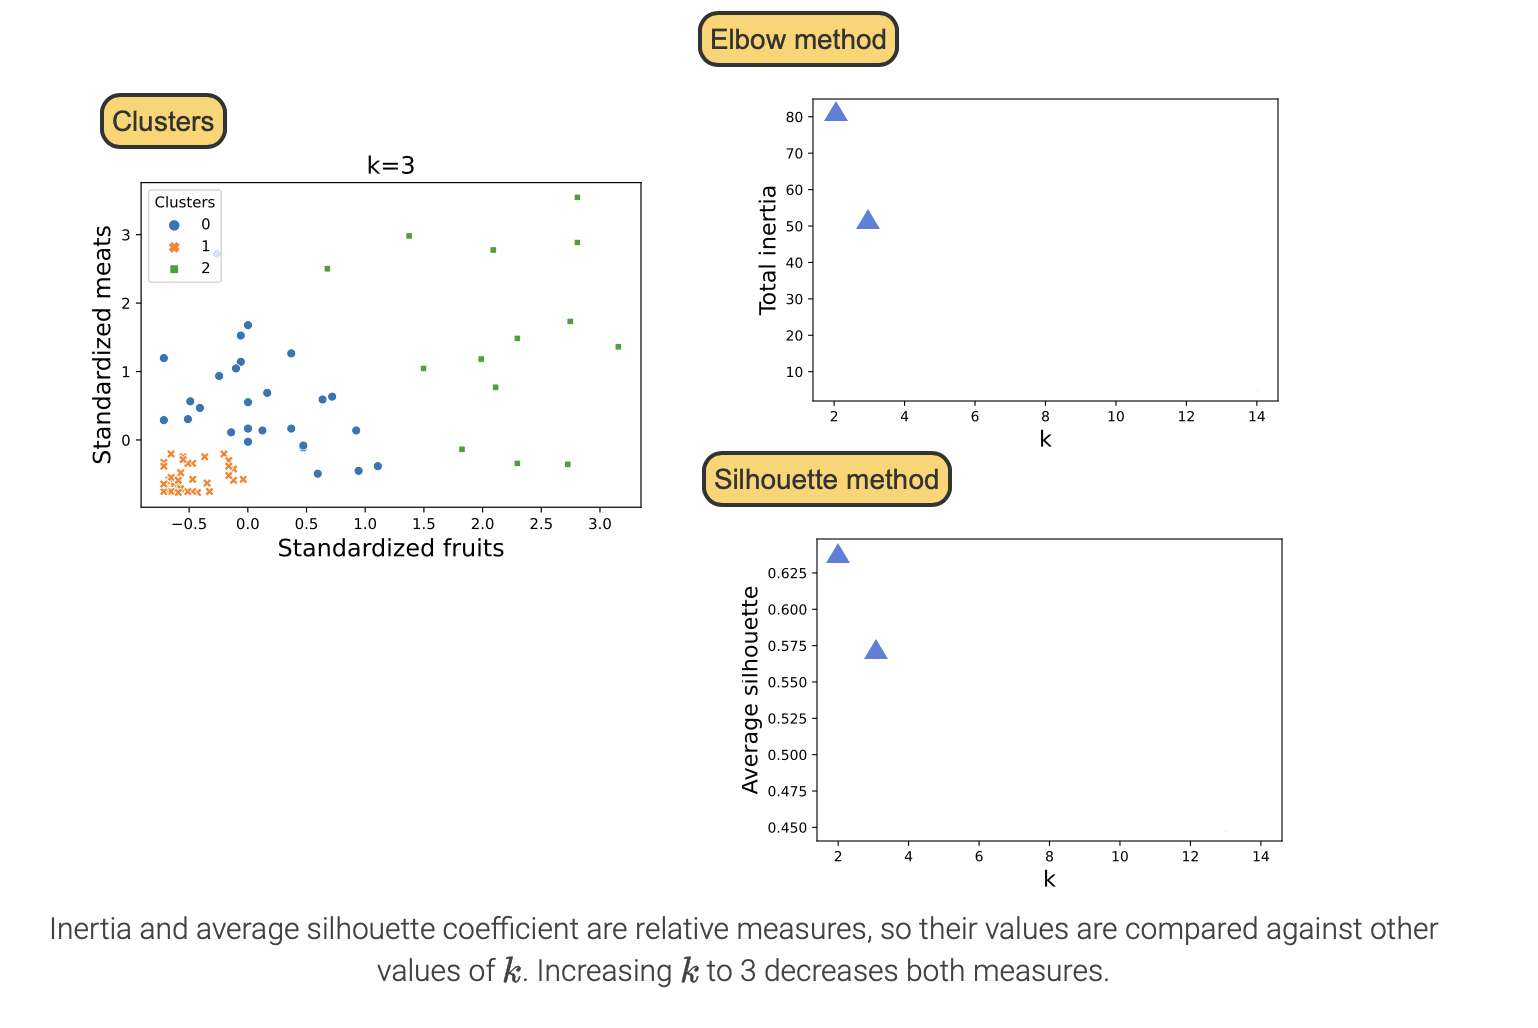
\includegraphics[width=0.8\textwidth]{imgs/k_mean_11.png}
    \end{figure}
\end{frame}

\begin{frame}
    \frametitle{Selecting the optimal number of clusters.}
    \begin{figure}[ht]
        \centering
        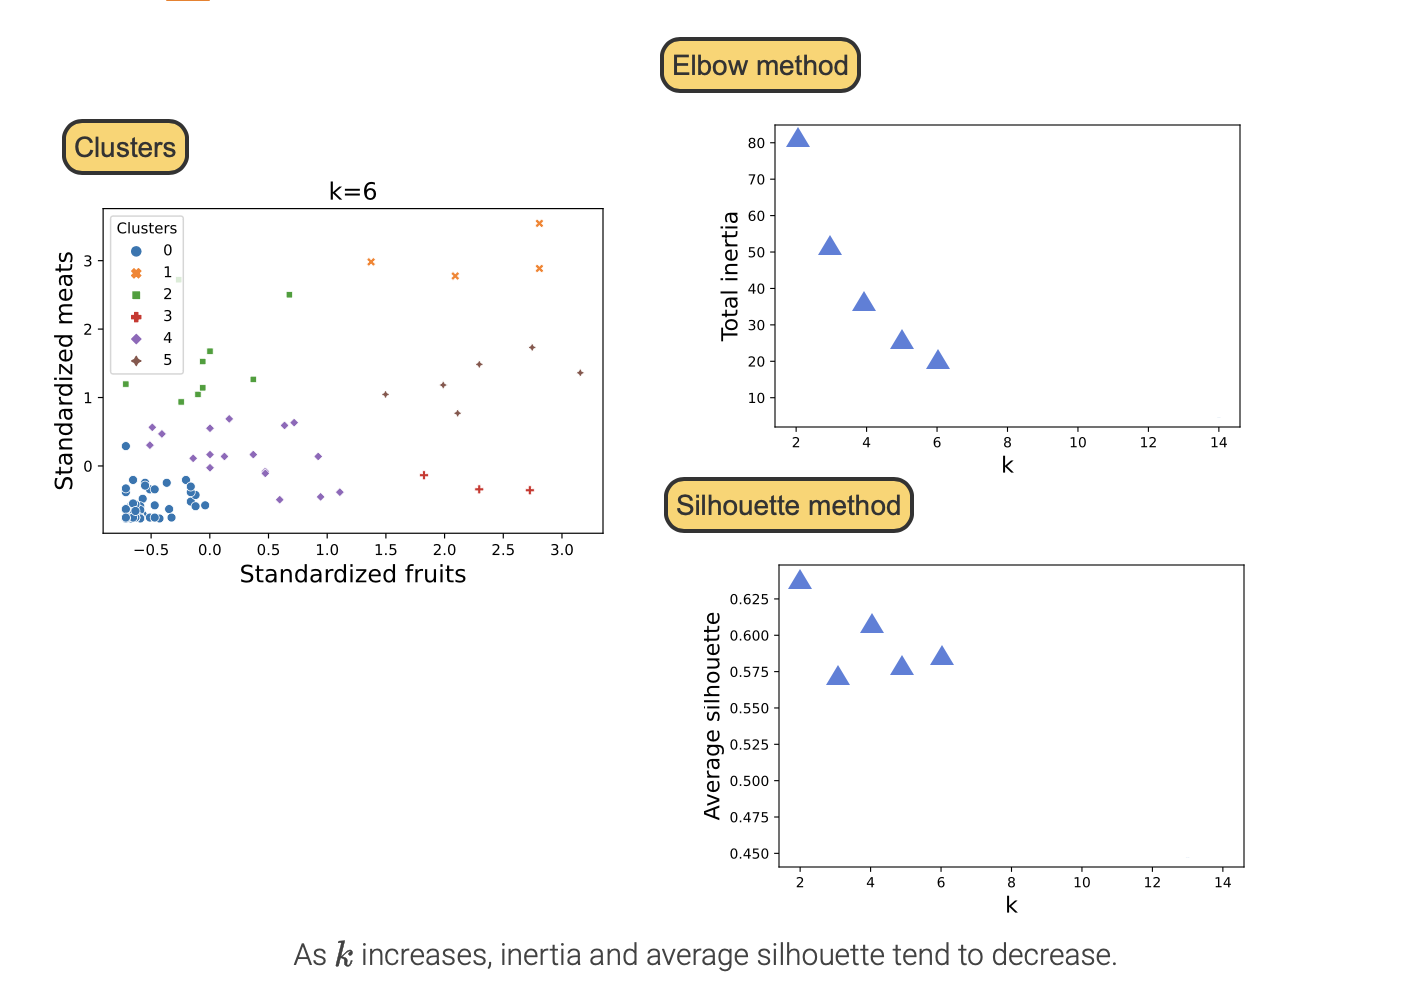
\includegraphics[width=0.8\textwidth]{imgs/k_mean_12.png}
    \end{figure}
\end{frame}

\begin{frame}
    \frametitle{Selecting the optimal number of clusters.}
    \begin{figure}[ht]
        \centering
        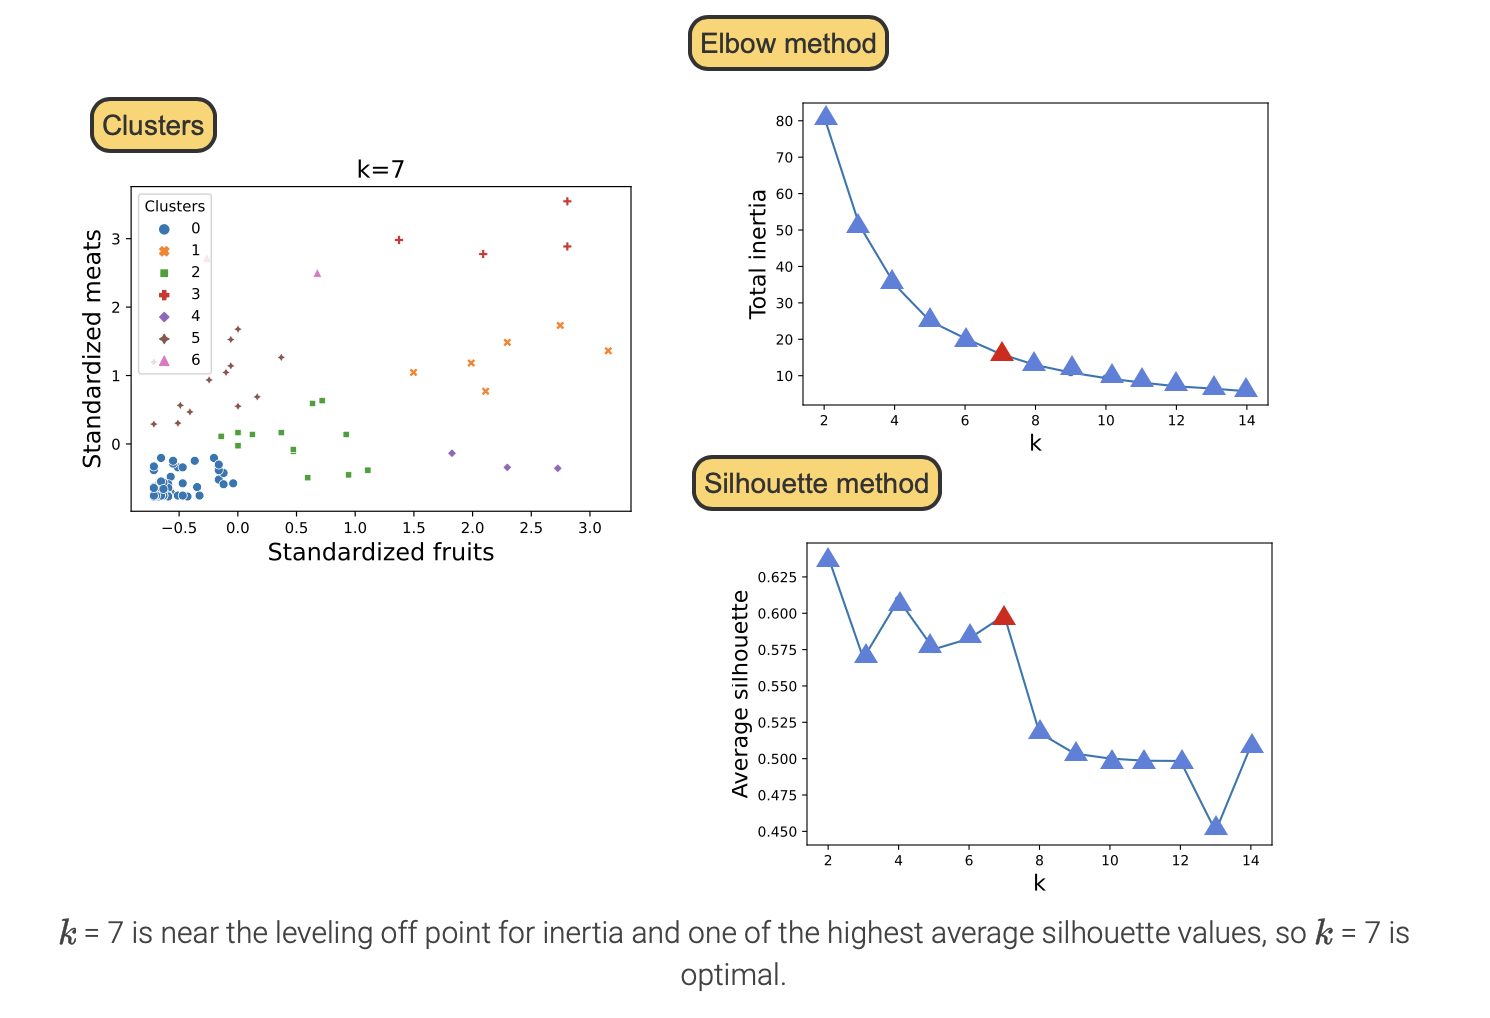
\includegraphics[width=0.8\textwidth]{imgs/k_mean_13.png}
    \end{figure}
\end{frame}

\begin{frame}
    \frametitle{Advantages and Disadvantages of K-means}
    k-means clustering works well for small and medium sized datasets where all clusters are about the same size. Since instances are assigned to clusters based on distances, all input features should be scaled before clustering.

    k-means clustering has several disadvantages:
    \begin{itemize}
        \item \textit{Correlation}: When input features are correlated, k-means clustering fails to identify reasonable clusters. Using principal components instead of the original features can improve interpretability and cluster separation.
    \end{itemize}
\end{frame}

\begin{frame}
    \frametitle{Advantages and Disadvantages of K-means}
    k-means clustering has several disadvantages:
    \begin{itemize}
        \item \textit{Correlation}: When input features are correlated, k-means clustering fails to identify reasonable clusters. Using principal components instead of the original features can improve interpretability and cluster separation.
        \item \textit{Variance}: k-means clustering assumes all features have the same variance. Standardization or normalization ensures all variances are equal.
        \item \textit{Cluster sizes}: k-means clustering favors clusters with approximately equal sizes. k-means clustering often groups small natural clusters together.
    \end{itemize}
\end{frame}

\begin{frame}
    \frametitle{Advantages and Disadvantages of K-means}
    \begin{itemize}
        \item \textit{Shape}: k-means clustering using Euclidean distance prefers clusters with spherical shape. Other distance measures or clustering methods should be used for irregularly shaped clusters.
        \item \textit{Initial centroids}: The initial centroids directly impact the final clusters.
    \end{itemize}
\end{frame}


\end{document}